\documentclass{article}
\usepackage{amsmath}
\usepackage{tikz}
\usetikzlibrary{arrows.meta}

\begin{document}

\author{Amarnath Patel}
\title{COT2000 Exam 4}
\date{\today}
\maketitle

\section*{Question 1}
(a) \[ \text{Yes, there are two circuits in G:} \]
   \[ C_1: v_1 \rightarrow v_2 \rightarrow v_3 \rightarrow v_1 \]
   \[ C_2: v_4 \rightarrow v_4 \text{ (self-loop)} \]

(b) 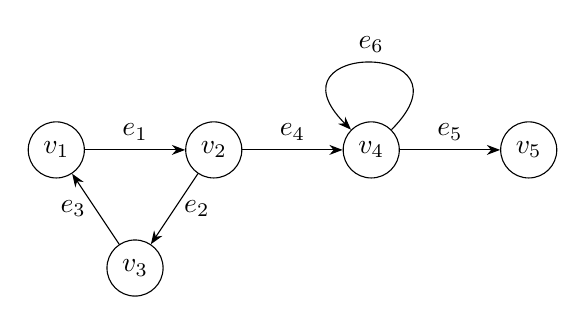
\begin{tikzpicture}[>={Stealth[]}]
    \node[draw,circle] (v1) at (0,0) {$v_1$};
    \node[draw,circle] (v2) at (2,0) {$v_2$};
    \node[draw,circle] (v3) at (1,-1.5) {$v_3$};
    \node[draw,circle] (v4) at (4,0) {$v_4$};
    \node[draw,circle] (v5) at (6,0) {$v_5$};
    
    \draw[->] (v1) -- node[above] {$e_1$} (v2);
    \draw[->] (v2) -- node[right] {$e_2$} (v3);
    \draw[->] (v3) -- node[left] {$e_3$} (v1);
    \draw[->] (v2) -- node[above] {$e_4$} (v4);
    \draw[->] (v4) -- node[above] {$e_5$} (v5);
    \draw[->] (v4) to[out=45,in=135,looseness=8] node[above] {$e_6$} (v4);
   \end{tikzpicture}

(c) \begin{align*}
    &\text{Vertex} &\text{In-degree} &\text{Out-degree} \\
    &v_1 &1 &1 \\
    &v_2 &1 &2 \\
    &v_3 &1 &1 \\
    &v_4 &2 &2 \\
    &v_5 &1 &0
   \end{align*}

(d) 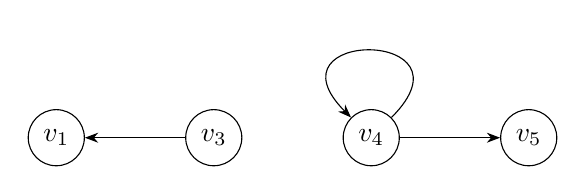
\begin{tikzpicture}[>={Stealth[]}]
    \node[draw,circle] (v1) at (0,0) {$v_1$};
    \node[draw,circle] (v3) at (2,0) {$v_3$};
    \node[draw,circle] (v4) at (4,0) {$v_4$};
    \node[draw,circle] (v5) at (6,0) {$v_5$};
    
    \draw[->] (v3) -- (v1);
    \draw[->] (v4) -- (v5);
    \draw[->] (v4) to[out=45,in=135,looseness=8] (v4);
   \end{tikzpicture}

(e) \[ \text{Yes, F has two connected components:} \]
   \[ \{v_1, v_3\} \text{ and } \{v_4, v_5\} \]


\section*{Question 2}

A multigraph is a graph that allows:
\begin{itemize}
    \item Multiple edges (parallel edges) between the same pair of vertices
    \item Loops (edges that connect a vertex to itself)
\end{itemize}

Differences from a simple graph:
\begin{itemize}
    \item Simple graphs do not allow parallel edges or loops
    \item In a simple graph, each edge is unique
    \item Multigraphs can have multiple edges with the same endpoints
\end{itemize}

\section*{Example Multigraph}

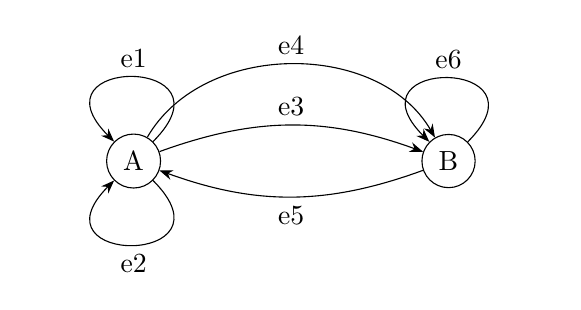
\begin{tikzpicture}[>={Stealth[]}]
    \node[draw,circle] (A) at (0,0) {A};
    \node[draw,circle] (B) at (4,0) {B};
    
    \draw[->] (A) to[out=45,in=135,looseness=8] node[above] {e1} (A);
    \draw[->] (A) to[out=315,in=225,looseness=8] node[below] {e2} (A);
    
    \draw[->] (A) to[bend left=20] node[above] {e3} (B);
    \draw[->] (A) to[bend left=60] node[above] {e4} (B);
    \draw[<-] (A) to[bend right=20] node[below] {e5} (B);
    
    \draw[->] (B) to[out=45,in=135,looseness=8] node[above] {e6} (B);
\end{tikzpicture}

\section*{Real-World Scenario}

This multigraph could represent a transportation network between two cities:

\begin{itemize}
    \item Vertices A and B represent two cities
    \item Edges represent different transportation routes:
    \begin{itemize}
        \item e1, e2: Local bus routes within city A
        \item e3: Highway from A to B
        \item e4: Train line from A to B
        \item e5: Flight from B to A
        \item e6: Local bus route within city B
    \end{itemize}
\end{itemize}

The multiple edges between A and B represent different modes of transportation, while the loops represent local transportation within each city.

\section*{Question 3}
(a) 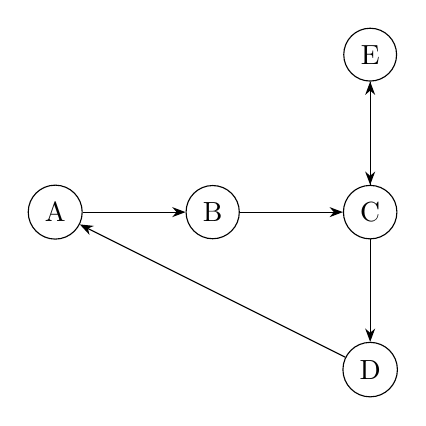
\begin{tikzpicture}[>={Stealth[]}, node distance=2cm]
    \node[draw,circle] (A) {A};
    \node[draw,circle] (B) [right of=A] {B};
    \node[draw,circle] (C) [right of=B] {C};
    \node[draw,circle] (D) [below of=C] {D};
    \node[draw,circle] (E) [above of=C] {E};
    
    \draw[->] (A) -- (B);
    \draw[->] (B) -- (C);
    \draw[->] (C) -- (D);
    \draw[->] (D) -- (A);
    \draw[->] (C) -- (E);
    \draw[->] (E) -- (C);
   \end{tikzpicture}

(b) Circuits in the graph:
   \begin{itemize}
    \item $A \rightarrow B \rightarrow C \rightarrow D \rightarrow A$ (Simple circuit)
    \item $C \rightarrow E \rightarrow C$ (Simple circuit)
   \end{itemize}

(c) This graph does not have an Euler path or circuit.

   Justification:
   \begin{itemize}
    \item For a directed graph to have an Euler circuit, every vertex must have equal in-degree and out-degree.
    \item For an Euler path, at most two vertices can have unequal in-degree and out-degree, differing by 1.
    \item In this graph:
      \begin{align*}
        &\text{Vertex} &\text{In-degree} &\text{Out-degree} \\
        &A &1 &1 \\
        &B &1 &1 \\
        &C &2 &2 \\
        &D &1 &1 \\
        &E &1 &1
      \end{align*}
    \item While the in-degrees and out-degrees are equal for each vertex, there are 6 edges but not all vertices are connected in a single circuit.
    \item The graph consists of two separate circuits that cannot be combined into a single Euler path or circuit.
   \end{itemize}

\section*{Question 4}
(a) Graphs G1 and G2:

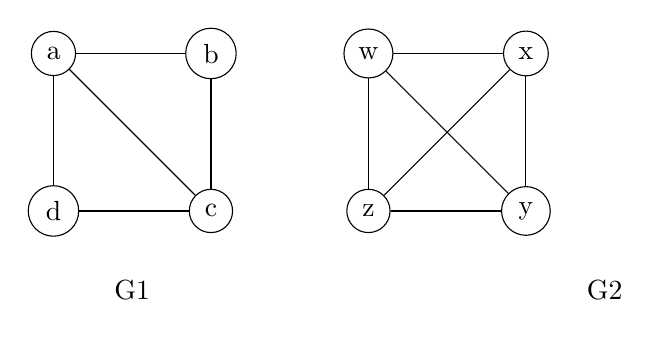
\begin{tikzpicture}[>={Stealth[]}, node distance=2cm]
    \node[draw,circle] (a) {a};
    \node[draw,circle] (b) [right of=a] {b};
    \node[draw,circle] (c) [below of=b] {c};
    \node[draw,circle] (d) [below of=a] {d};
    
    \draw (a) -- (b);
    \draw (b) -- (c);
    \draw (c) -- (d);
    \draw (d) -- (a);
    \draw (a) -- (c);
    
    \node[draw,circle] (w) at ([xshift=4cm]a.center) {w};
    \node[draw,circle] (x) [right of=w] {x};
    \node[draw,circle] (y) [below of=x] {y};
    \node[draw,circle] (z) [below of=w] {z};
    
    \draw (w) -- (x);
    \draw (x) -- (y);
    \draw (y) -- (z);
    \draw (z) -- (w);
    \draw (w) -- (y);
    \draw (x) -- (z);
    
    \node at (1,-3) {G1};
    \node at (7,-3) {G2};
\end{tikzpicture}

(b) Isomorphism analysis:

i. Vertex mapping function $f : V(G1) \rightarrow V(G2)$:
   \begin{align*}
   f(a) &= w \\
   f(b) &= x \\
   f(c) &= y \\
   f(d) &= z
   \end{align*}

ii. Edge mapping function $h : E(G1) \rightarrow E(G2)$:
    \begin{align*}
    h(a,b) &= (w,x) \\
    h(b,c) &= (x,y) \\
    h(c,d) &= (y,z) \\
    h(d,a) &= (z,w) \\
    h(a,c) &= (w,y)
    \end{align*}

iii. Verification of one-to-one correspondence:

For each edge $e = (u,v)$ in $E(G1)$, we confirm $h(e) = (f(u), f(v))$ in $E(G2)$:

\begin{align*}
h(a,b) &= (f(a), f(b)) = (w,x) \in E(G2) \\
h(b,c) &= (f(b), f(c)) = (x,y) \in E(G2) \\
h(c,d) &= (f(c), f(d)) = (y,z) \in E(G2) \\
h(d,a) &= (f(d), f(a)) = (z,w) \in E(G2) \\
h(a,c) &= (f(a), f(c)) = (w,y) \in E(G2)
\end{align*}

However, G1 and G2 are not isomorphic because:
\begin{itemize}
\item G2 has an additional edge $(x,z)$ that doesn't correspond to any edge in G1.
\item The degree sequences differ: G1 has [3,2,3,2] and G2 has [3,3,3,3].
\end{itemize}

Therefore, while we can define functions $f$ and $h$, they do not establish an isomorphism between G1 and G2.

\section*{Question 5}

\subsection*{a) Isomorphism}

G1 and G2 are not isomorphic:
\begin{itemize}
  \item Vertices: G1 (6), G2 (6)
  \item Edges: G1 (7), G2 (7)
  \item Degree sequences differ:
    \begin{itemize}
      \item G1: [2, 3, 5, 1, 1, 2]
      \item G2: [2, 1, 5, 2, 3, 1]
    \end{itemize}
\end{itemize}

\subsection*{b) Adjacency Matrix G1}

\[
\begin{pmatrix}
0 & 1 & 1 & 0 & 0 & 0 \\
1 & 0 & 1 & 0 & 0 & 1 \\
1 & 1 & 0 & 1 & 1 & 1 \\
0 & 0 & 1 & 0 & 0 & 0 \\
0 & 0 & 1 & 0 & 0 & 0 \\
0 & 1 & 1 & 0 & 0 & 0
\end{pmatrix}
\]

\subsection*{c) Adjacency Matrix G2}

\[
\begin{pmatrix}
0 & 0 & 1 & 0 & 1 & 0 \\
0 & 0 & 1 & 0 & 0 & 0 \\
1 & 1 & 0 & 1 & 1 & 1 \\
0 & 0 & 1 & 0 & 1 & 0 \\
1 & 0 & 1 & 1 & 0 & 0 \\
0 & 0 & 1 & 0 & 0 & 0
\end{pmatrix}
\]

\subsection*{d) Vertex Degrees}

G1: $\{2, 3, 5, 1, 1, 2\}$

G2: $\{2, 1, 5, 2, 3, 1\}$

\section*{Question 6}

\subsection*{(a) Isomorphic Subgraphs}

G1 adjacency matrix:
\[
\begin{pmatrix}
0 & 1 & 0 \\
1 & 0 & 1 \\
0 & 1 & 0
\end{pmatrix}
\]

G2 adjacency matrix:
\[
\begin{pmatrix}
0 & 1 & 0 & 0 \\
1 & 0 & 1 & 0 \\
0 & 1 & 0 & 1 \\
0 & 0 & 1 & 0
\end{pmatrix}
\]

Process:
\begin{itemize}
\item Examine all 3x3 submatrices of G2
\item Compare each to G1's matrix
\item Count isomorphic subgraphs
\end{itemize}

Result: 2 isomorphic subgraphs

\subsection*{(b) Graph Drawings}

\begin{tikzpicture}[node distance=2cm]
\node[draw,circle] (1) at (0,0) {1};
\node[draw,circle] (2) at (2,0) {2};
\node[draw,circle] (3) at (1,-1.5) {3};
\draw (1) -- (2);
\draw (2) -- (3);
\node at (1,-2.5) {G1};

\node[draw,circle] (A) at (5,0) {1};
\node[draw,circle] (B) at (7,0) {2};
\node[draw,circle] (C) at (9,0) {3};
\node[draw,circle] (D) at (7,-1.5) {4};
\draw (A) -- (B);
\draw (B) -- (C);
\draw (C) -- (D);
\node at (7,-2.5) {G2};
\end{tikzpicture}

\end{document}